\section{Data Pipeline: From Examination Documents to 1,202 Serviceable Items}
\label{sec:data-pipeline}

\subsection{The pipeline}
The item bank is not authored; it is \emph{recovered}. The public Shanghai chemistry examinations (155 distinct papers in the bank's ledger) yield 6,083 raw item slices (\path{data/raw_papers/shanghai_all.jsonl}); their official answer keys are public. We build a deterministic pipeline from the original Word files to block-structured items:

\begin{enumerate}\setlength{\itemsep}{0pt}\setlength{\parskip}{0pt}\setlength{\parsep}{0pt}
\item \textbf{Source inventory}: the bank's 3,329 structured items each carry a \texttt{source\_path} pointing to a Word document (.docx/.doc): 3,329/3,329 coverage, 155 distinct papers (\texttt{group\_key}s).
\item \textbf{Extraction}: python-docx for text flow; DWML for OMML$\rightarrow$LaTeX; OLE+WMF rendering; direct \texttt{word/media} asset extraction; {answer}/{solution} anchors serve as natural cut points to separate stem, answer, and solution blocks.
\item \textbf{Block schema v4}: \texttt{text / latex / chem / figure / table} block types; answer blocks stored separately from the stem.
\item \textbf{Ground truth}: a 60-question gold set (50 formal + 10 reserve) anchored to official keys; gold labels held privately by the auditor, producer blind. Asset-level gold: 68 images (34 calibration + 34 blind) with blind-run comparison.
\item \textbf{Result}: 3,329 items with globally unique IDs, schema \texttt{ws3\_schema\_v4\_candidate\_1}, plus 10,102 asset transcript rows (5,552 formula-LaTeX, 2,683 ai\_seed, 1,595 display-only, 271 manual-queue, 1 leak-rejected) and 13,171 media-reference rows.
\end{enumerate}

\begin{figure}[t]
\centering
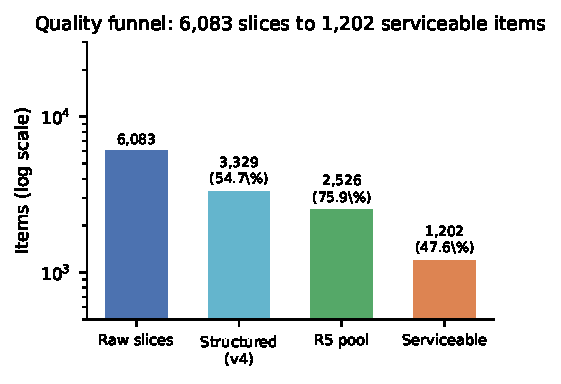
\includegraphics[width=0.62\textwidth]{figures/fig2_funnel.pdf}
\caption{The quality funnel: from 6,083 raw slices of 155 source papers to 1,202 serviceable items. Labels show yields relative to the previous stage.}
\label{fig:funnel}
\end{figure}
\subsection{The QA marathon: 2,526 to 1,202 (47.6\%)}
Figure~\ref{fig:funnel} visualizes the funnel. Ten batches (BATCH6, BATCH8--16; the continuous numbering from BATCH6 has a gap where batch 7 was not archived under that name) audited the recovered pool under one acceptance line: \emph{a student must be able to use the item}. The funnel:

\begin{table}[h]
\centering
\small
\begin{tabular}{lrl}
\toprule
\textbf{Stage} & \textbf{Count} & \textbf{Note} \\
\midrule
Examination papers (ledger) & 155 & distinct \texttt{group\_key}s \\
Raw item slices & 6,083 & \texttt{shanghai\_all.jsonl} \\
Structured items (v4) & 3,329 & unique IDs \\
Usability candidate pool & 2,526 & R5 ledger \\
\textbf{Serviceable (r5\_serve=true)} & \textbf{1,202} & 47.6\% of candidate pool \\
\bottomrule
\end{tabular}
\caption{The quality funnel. A raw-slice to serviceable-item yield of 19.8\%.}
\label{tab:funnel}
\end{table}

Three methodological findings came out of this marathon, each with a concrete incident:

\begin{enumerate}\setlength{\itemsep}{0pt}\setlength{\parskip}{0pt}\setlength{\parsep}{0pt}
\item \textbf{Rendering without crashing $\neq$ item usable.} The first acceptance attempt verified only ``the render pipeline does not throw''; the user review failed it (missing figures, empty answers, broken ions). The usable-item ledger became an on-line gate.
\item \textbf{The auditor must see what students see.}\label{it:auditor-sameness} The screenshot pipeline ran without KaTeX for an entire batch; the vision-language channel judged a different product than the browser. Fix: same-source verification before auditing.
\item \textbf{Precision gold must accompany recall gold.} A new five-dimension reviewer was calibrated only on known-bad items and later misflagged 169 good items in the whitelist ($\approx$13\% of the whitelist). Node-aware text scanning (sentinels for formula/media/omml) fixed it: 0 false positives on 1,207 whitelist rows, and R5 exclusions were re-verified.
\end{enumerate}

Quantified costs: the full-pool vision-language audit of the 2,526 pool cost \textyen17.93; the hardest batch (batch13, ``dead figure'' recovery) rescued 105 assets for \textyen2.53. A P0 hazard was also found and fixed on-line: crop images included printed answers from the original paper, so an OCR answer-leak gate became part of the accept line (Section~\ref{sec:governance}).

\subsection{What the numbers say}
The raw-to-serviceable yield is 19.8\%. This is the \emph{price} of evidence-binding in the data sense: producing a bank where every item's answer is verifiable, its figure is renderable, and its provenance is traceable, costs most of the pool. The 2026-09 file snapshot changed two figures relative to the published white paper (WS2 transcript rows 10,102 and media-ref rows 13,171, vs.\ 6,005 and 12,790 in the earlier report)---a directly measurable consequence of later batch recovery; we report current-tree values as canonical.

\subsection{What is \emph{not} demonstrated}
This pipeline produces a \emph{constructible} bank, not a \emph{validated} one: no student answered any of these items in a controlled setting; no item-difficulty calibration exists beyond the examination's own implicit design; and 926 of 3,329 items lack an \path{answer_source_path} (27.8\%), meaning those items' standard answers rest on the document's answer block alone.
